\documentclass[a4paper, top=10mm]{article}
%for writing from the top
\usepackage{fullpage}
%for math
\usepackage{amsmath}
\usepackage{mathrsfs}
\usepackage{amsthm}
\usepackage{amsfonts}
%for images
\usepackage{graphicx}
%for links
\usepackage{hyperref}
%for color
\usepackage{xcolor}
%for title
\title{\textbf{\huge{The Bézier Curve}}}
\author{Enigma n\textsuperscript{o}9}
\date{2\textsuperscript{nd} December 2022}

\newtheorem*{hint}{Hint}

\addtolength{\voffset}{-2cm}
\addtolength{\textheight}{5cm}


\begin{document}
	\maketitle
	
	Bézier curve is named after French engineer Pierre Bézier, who used it in the 1960s for designing curves for the bodywork of Renault cars.
	Other uses include the design of computer fonts and animation.
	
	Bézier curves are defined as follows:\\
	Let $B_{P_1 \dots P_k}$ denote the Bézier curve determined by any selection of points $P_1, \dots, P_k$.
	Then we define recursively:
	$$B_{P_1}(t) = P_1 \text{ and } B(t) = B_{P_1 \dots P_n}(t) = (1-t) B_{P_1 \dots P_{n-1}}(t) + t B_{P_1 \dots P_{n-1}}(t)$$

	Let the eight points $P_1, \dots, P_8$ be defined as follows:
	\begin{itemize}
		\item $P_1$ $(0,0)$
		\item $P_2$ $(-2,2)$
		\item $P_3$ $(0,3)$
		\item $P_4$ $(-1,0)$
		\item $P_5$ $(1,0)$
		\item $P_6$ $(0,3)$
		\item $P_7$ $(2,2)$
		\item $P_8$ $(0,0)$
	\end{itemize}
	
	\begin{center}
		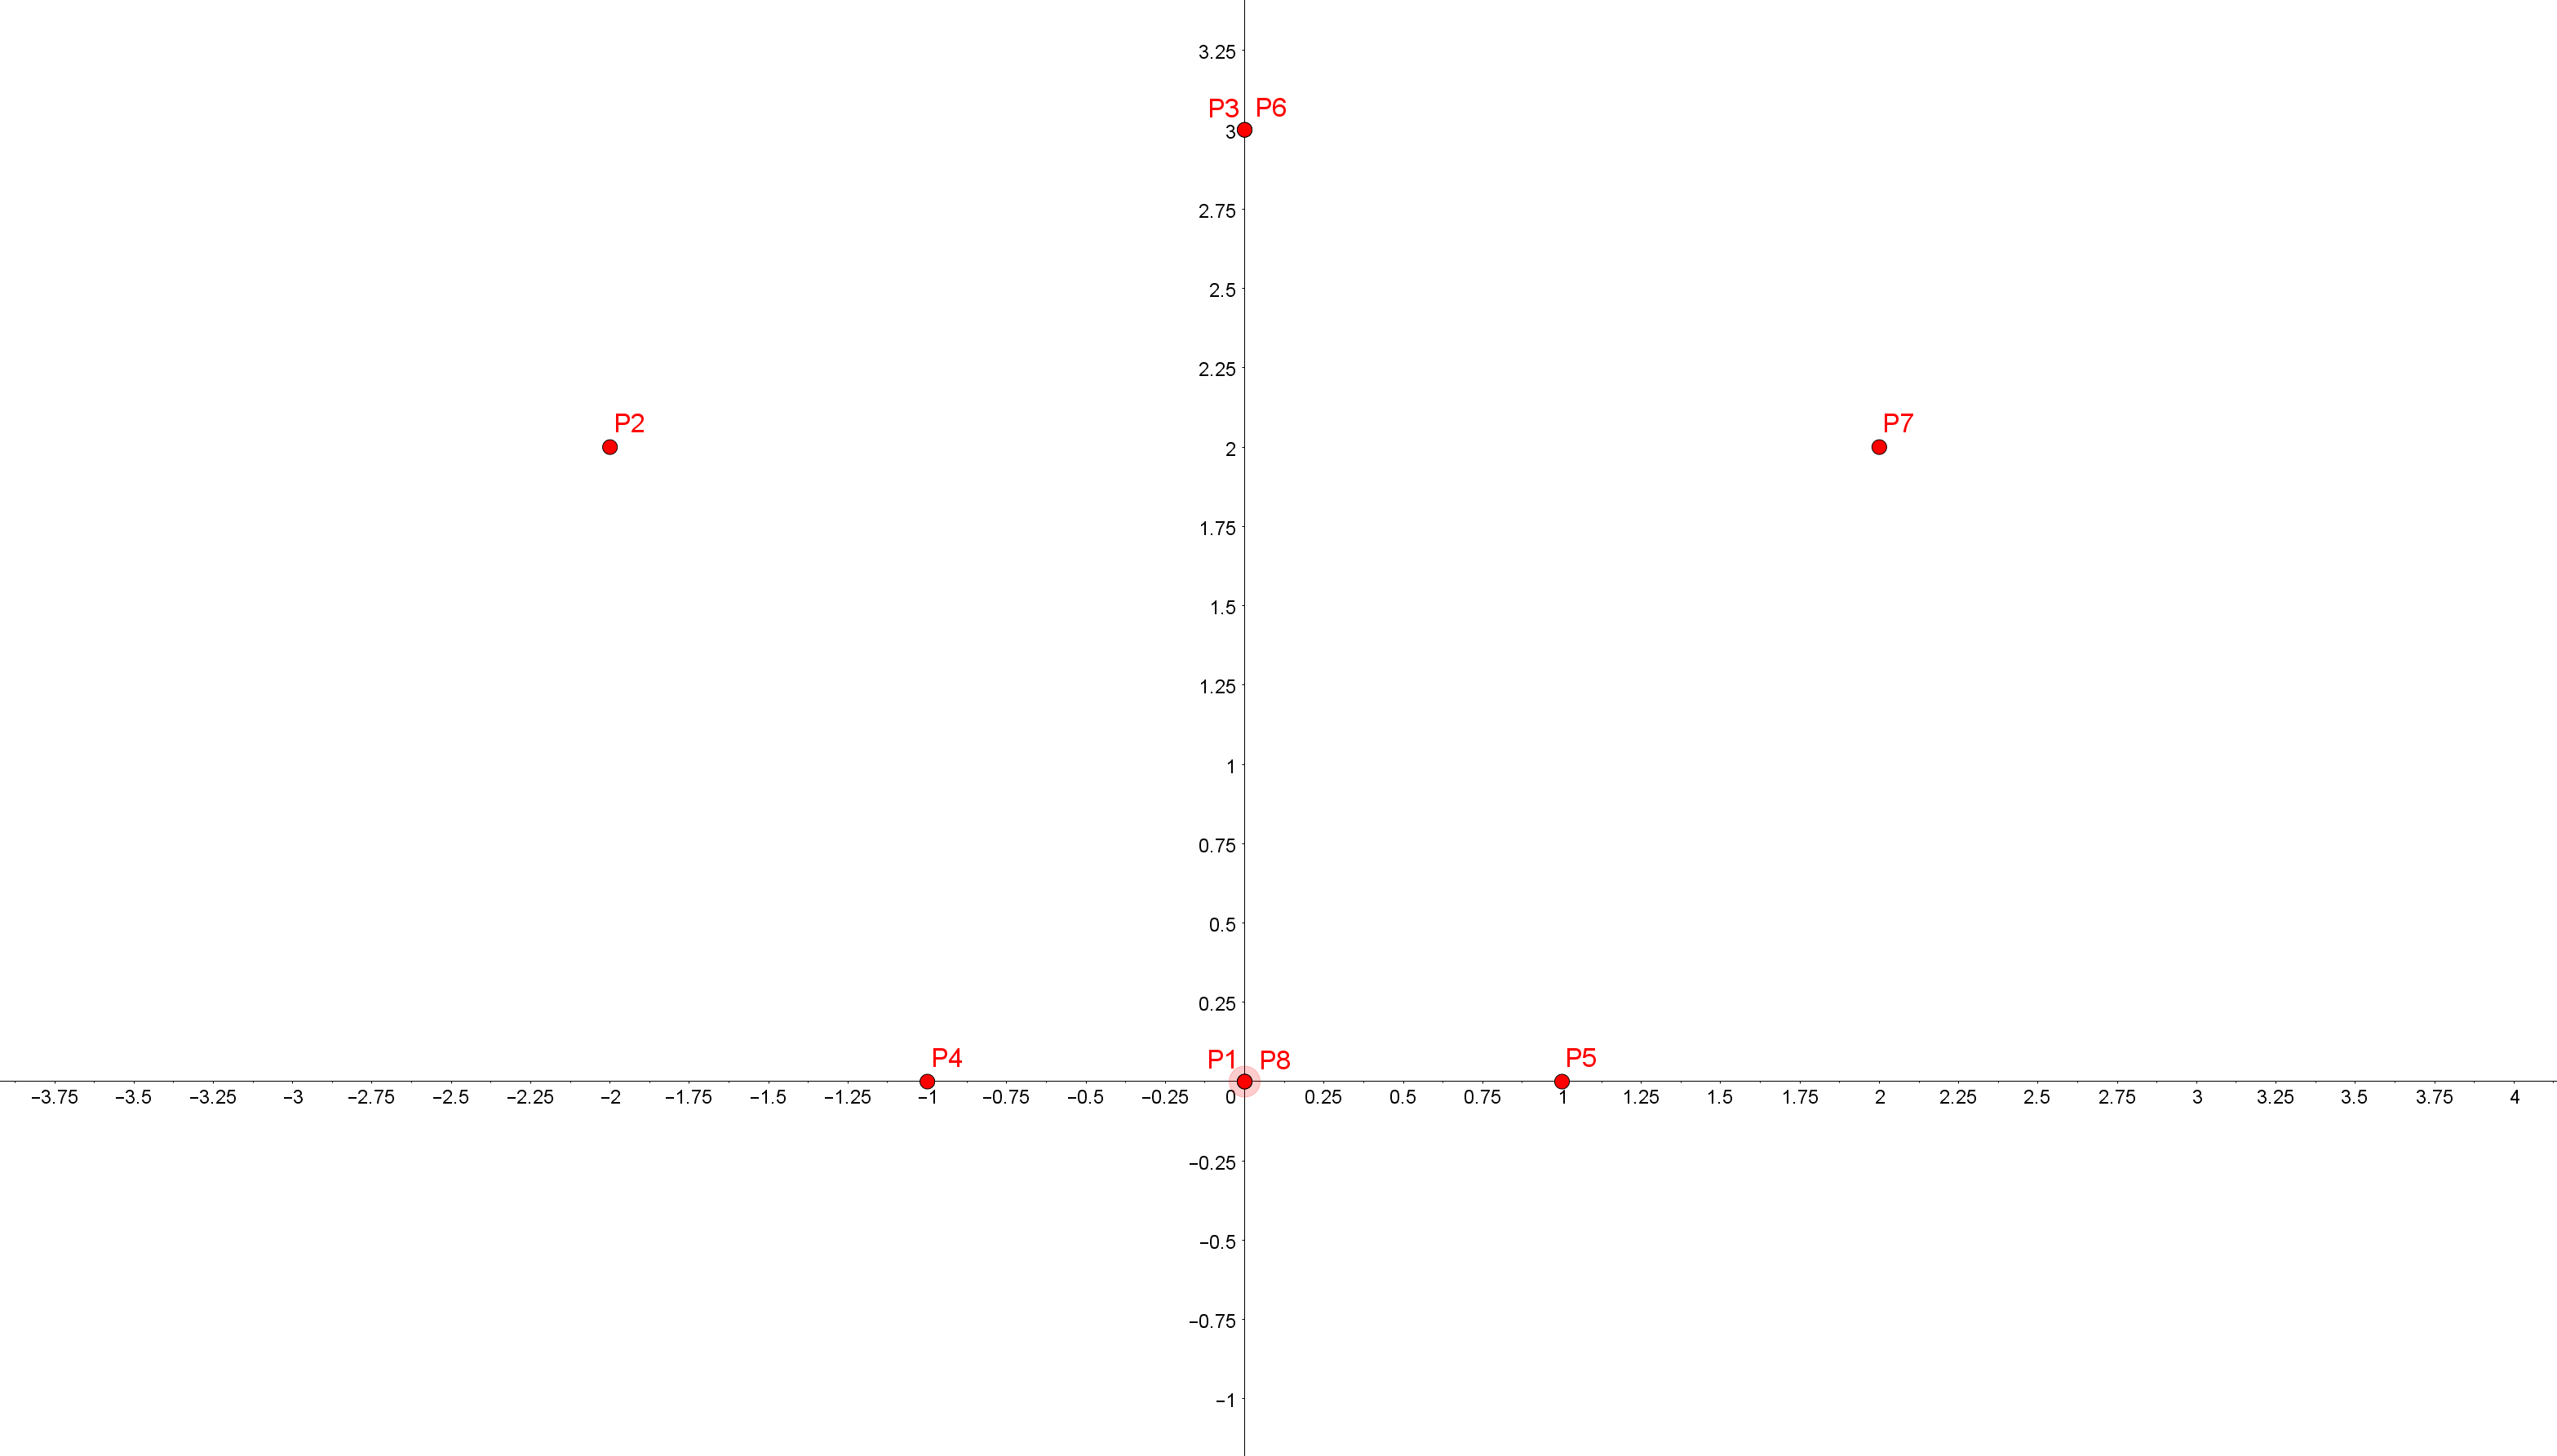
\includegraphics[height=200pt]{09points.png}
	\end{center}
	
	\textbf{What is the name of the shape given by tracing the Bézier curve with the eight point given above?}

	\vspace{2cm}
	
	You may want to use \url{https://pauldubois98.github.io/MathCurves/BezierCurves/} to plot Bézier curves easily, or scan the QR code below:
	\begin{center}
		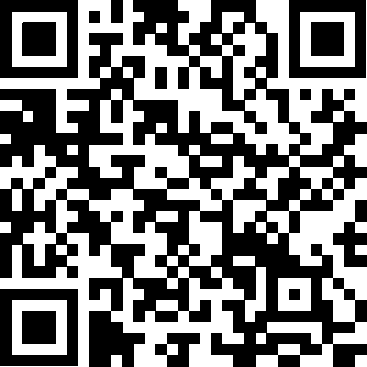
\includegraphics[height=100pt]{09QR_Bezier.png}
	\end{center}
	
	% plot solution: https://pauldubois98.github.io/MathCurves/BezierCurves/index.html?n=8&t=0&animation=on&xs=[300,50,300,175,425,300,550,300]&ys=[390,140,15,390,390,15,140,390]
	
\end{document}